\documentclass[10pt]{article}
\usepackage[a4paper, margin=2cm]{geometry}
\usepackage[utf8]{inputenc}
\usepackage{graphicx}
\usepackage{lastpage}
\usepackage{fancyhdr}

\pagestyle{fancy}
\fancyhf{}
\rfoot{Page \thepage \hspace{1pt} sur \pageref{LastPage}}

\begin{document}

\title{Math - Devoir Formatif}
\author{Hovinne Noé}
\date{}
\maketitle
\section*{Exercice 42 (p. 161) : château d'eau}\vspace{0.2cm}

%----------------------------------------------------------------------------------------------------------------------------------------
\flushleft Le réservoir sphérique d'un château d'eau a un rayon de 6 $m$.

a. Calculer, en $m^3$, la capacité maximum de ce réservoir.

$$V = {\pi \times 4R^2\over{3}} = {\pi \times 4.6^2\over{3}} = 904,77 m^3$$\vspace{0.1cm}

b. Calculer, en $m^3$, le volume d'eau contenu dans la partie sphérique de ce réservoir lorsque la hauteur de l'eau y est

\hspace{1cm}1) de 4 $m$ ;

$$V=\pi \times \int\limits_{-6}^{-2} \left( \sqrt{6^2-x^2} \right)^2dx$$
$$=\pi \times \int\limits_{-6}^{-2} (36-x^2)dx$$
$$=\pi \times \left[ 36x-{x^3\over{3}} \right]_{-6}^{-2}$$
$$=\pi \times \frac{224}{3}$$
$$=234,572251 m^3$$

\hspace{1cm}2) de 7 $m$ ;

$$V=\pi \times \int\limits_{-6}^{1} \left( \sqrt{6^2-x^2} \right)^2dx$$
$$=\pi \times \int\limits_{-6}^{1} (36-x^2)dx$$
$$=\pi \times \left[ 36x-{x^3\over{3}} \right]_{-6}^{1}$$
$$=\pi \times \frac{539}{3}$$
$$=564,4394801 m^3$$

\newpage

\hspace{1cm}3) de $x$ $m$ ($0 \leq x \leq 12$).

$$V=\pi \times \int\limits_{-6}^{x-6} \left( \sqrt{6^2-x^2} \right)^2dx$$
$$=\pi \times \int\limits_{-6}^{x-6} (36-x^2)dx$$
$$=\pi \times \left[ 36x-{x^3\over{3}} \right]_{-6}^{x-6}$$
$$=\pi \times \left( -\frac{(x-6)^3}{3}+36x-72 \right)$$

\begin{figure}[h]
    \textit{\caption{$f(x)=\sqrt{36-x^2}$}}\vspace{1cm}
    \centering
    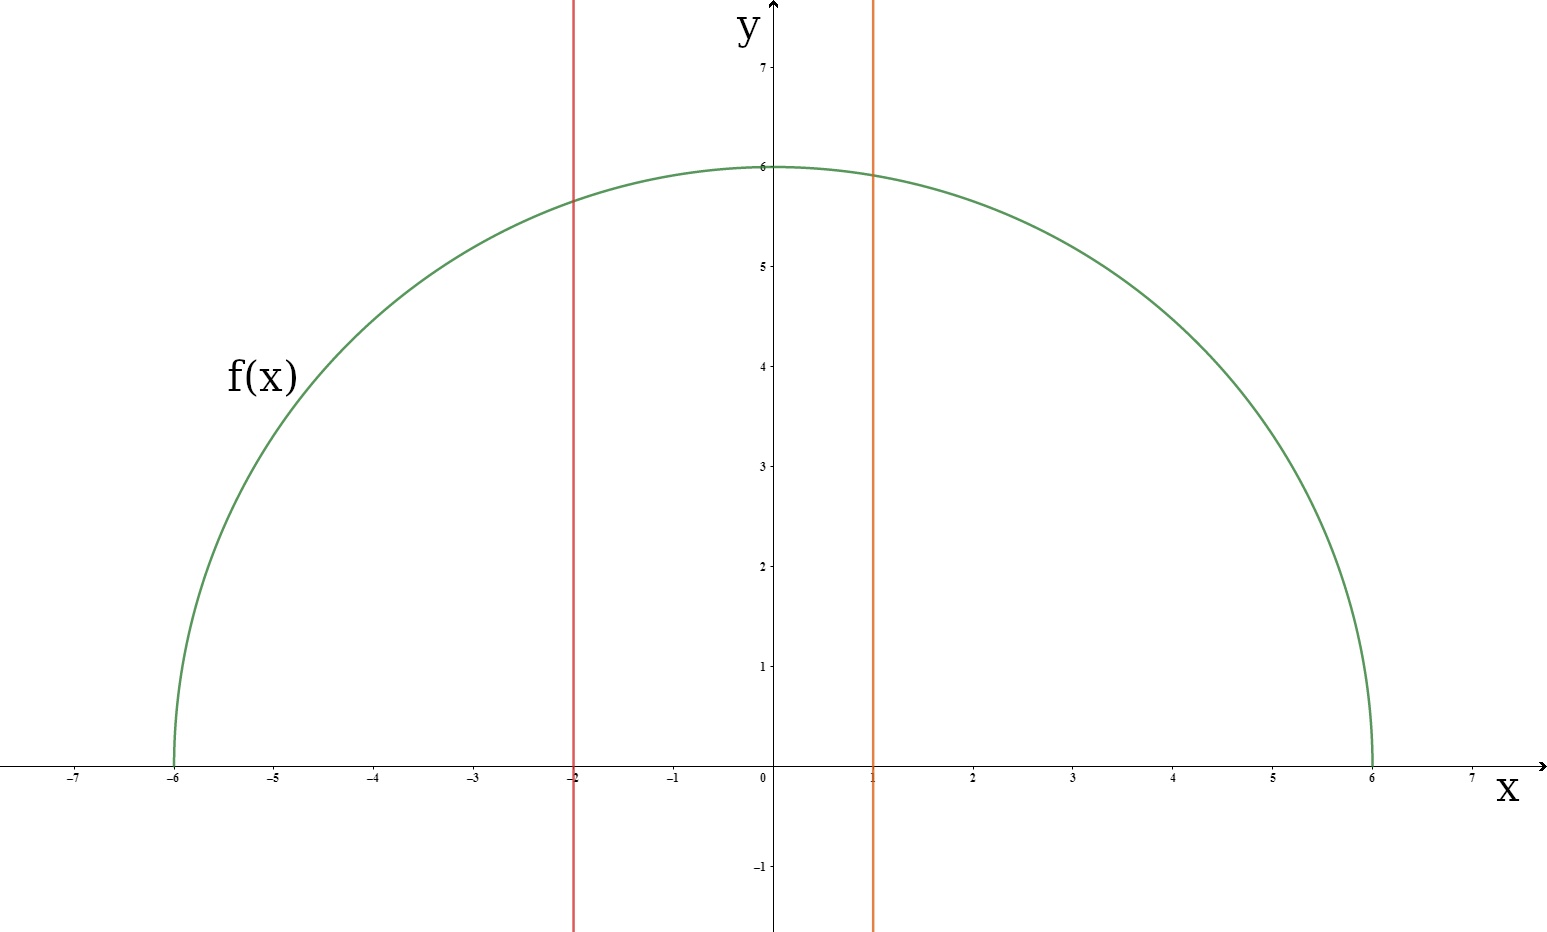
\includegraphics[width=16cm, height=10cm]{assets/ex42-schema.png}
\end{figure}\vspace{4cm}
%----------------------------------------------------------------------------------------------------------------------------------------
\begin{center}
\vspace{1cm}Réalisé en \LaTeX\vspace{0.2cm}

Code source : https://github.com/noehov/coursmath6
\end{center}
%----------------------------------------------------------------------------------------------------------------------------------------
\end{document}